\documentclass[tikz,border=6pt]{standalone}
\usepackage[T1]{fontenc}
\usepackage[utf8]{inputenc}
\usepackage{pgfplots}
\usepgfplotslibrary{groupplots}
\usetikzlibrary{calc}
\pgfplotsset{compat=1.18}
\begin{document}
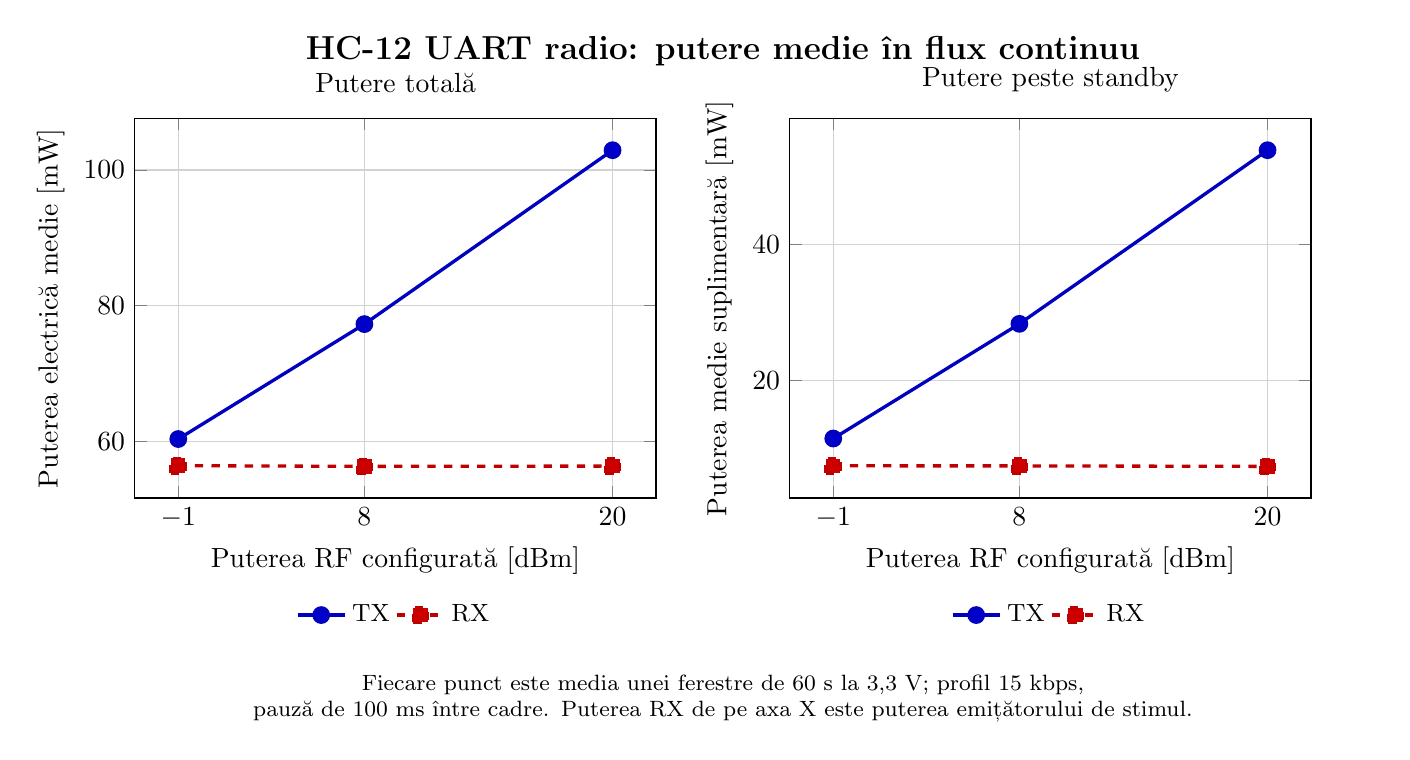
\begin{tikzpicture}
\begin{groupplot}[/pgf/number format/use comma,
  group style={group size=2 by 1, horizontal sep=1.7cm},
  width=8.2cm, height=6.4cm,
  xmin=-3.1, xmax=22.1, xtick={-1,8,20},
  xlabel={Puterea RF configurată [dBm]},
  grid=both, minor grid style={gray!15}, major grid style={gray!35},
  every axis plot/.append style={line width=1.2pt, mark size=2.6pt},
  legend style={font=\small, draw=none, fill=none,
    at={(0.5,-0.25)}, anchor=north, legend columns=2},
]
\nextgroupplot[title={Putere totală}, ylabel={Puterea electrică medie [mW]}]
\addplot+[blue!75!black, mark=*] coordinates {(-1,60.3741983) (8,77.2986309) (20,102.909297)};
\addlegendentry{TX}
\addplot+[red!75!black, dashed, mark=square*] coordinates {(-1,56.4476364) (8,56.3466338) (20,56.3904428)};
\addlegendentry{RX}
\nextgroupplot[title={Putere peste standby}, ylabel={Puterea medie suplimentară [mW]}]
\addplot+[blue!75!black, mark=*] coordinates {(-1,11.418344) (8,28.319074) (20,53.9066183)};
\addlegendentry{TX}
\addplot+[red!75!black, dashed, mark=square*] coordinates {(-1,7.39785552) (8,7.38380049) (20,7.31445616)};
\addlegendentry{RX}
\end{groupplot}
\node[font=\bfseries\large] at ($(group c1r1.north)!0.5!(group c2r1.north)+(0,0.85cm)$)
  {HC-12 UART radio: putere medie în flux continuu};
\node[font=\footnotesize, align=center, text width=16.5cm]
  at ($(group c1r1.south)!0.5!(group c2r1.south)+(0,-2.55cm)$)
  {Fiecare punct este media unei ferestre de 60 s la 3,3 V; profil 15 kbps,\\
   pauză de 100 ms între cadre. Puterea RX de pe axa X este puterea emițătorului de stimul.};
\end{tikzpicture}
\end{document}
